\chapter{Binaire vloeistof-dampdiagrammen en destillatie}\label{ch:b2:liquid-vapour-diagrams}

Een koperen distilleerketel maakt van een wijn met een paar procent alcohol een
gedistilleerde drank die vele malen sterker is; een raffinaderijkolom splitst ruwe aardolie in fracties, van gas tot
zware stookolie. Beide berusten op één feit: de damp boven een kokend mengsel is
rijker aan het vluchtigste bestanddeel dan de vloeistof. Herhaal het
verdampen en condenseren vaak genoeg en de scheiding wordt zo scherp als
gewenst --- met één uitzondering: geen enkele destillatie, hoe lang de
kolom ook is, brengt ethanol boven ongeveer 95 massaprocent. Dit hoofdstuk tekent
de diagrammen die zeggen hoe een mengsel van twee vloeistoffen kookt, en gebruikt ze om
een kolom te ontwerpen en te zien waar ze moet ophouden.

\begin{recall}
\Cref{ch:b2:chemical-potential}: de \omterm{def:b2:chemical-potential:chemical-potential}{chemische potentiaal}, de \omterm{thm:b2:chemical-potential:raoult}{wet van Raoult} en het
ideale mengsel, \omterm{def:b2:chemical-potential:activity-coefficient}{activiteitscoëfficiënten} en afwijkingen van de \omterm{thm:b2:chemical-potential:raoult}{wet van Raoult}, de
betrekking van Gibbs--Duhem. \Cref{ch:b2:equilibrium-shifts}: de \omterm{def:b2:equilibrium-shifts:variance}{variantie}. Het
deel van jaar~1, over laboratoriumtechnieken: eenvoudige destillatie, mengbare en
niet-mengbare vloeistoffen. Het schoolboek: destillatie en hydrodestillatie.
\end{recall}

\begin{omfigure}
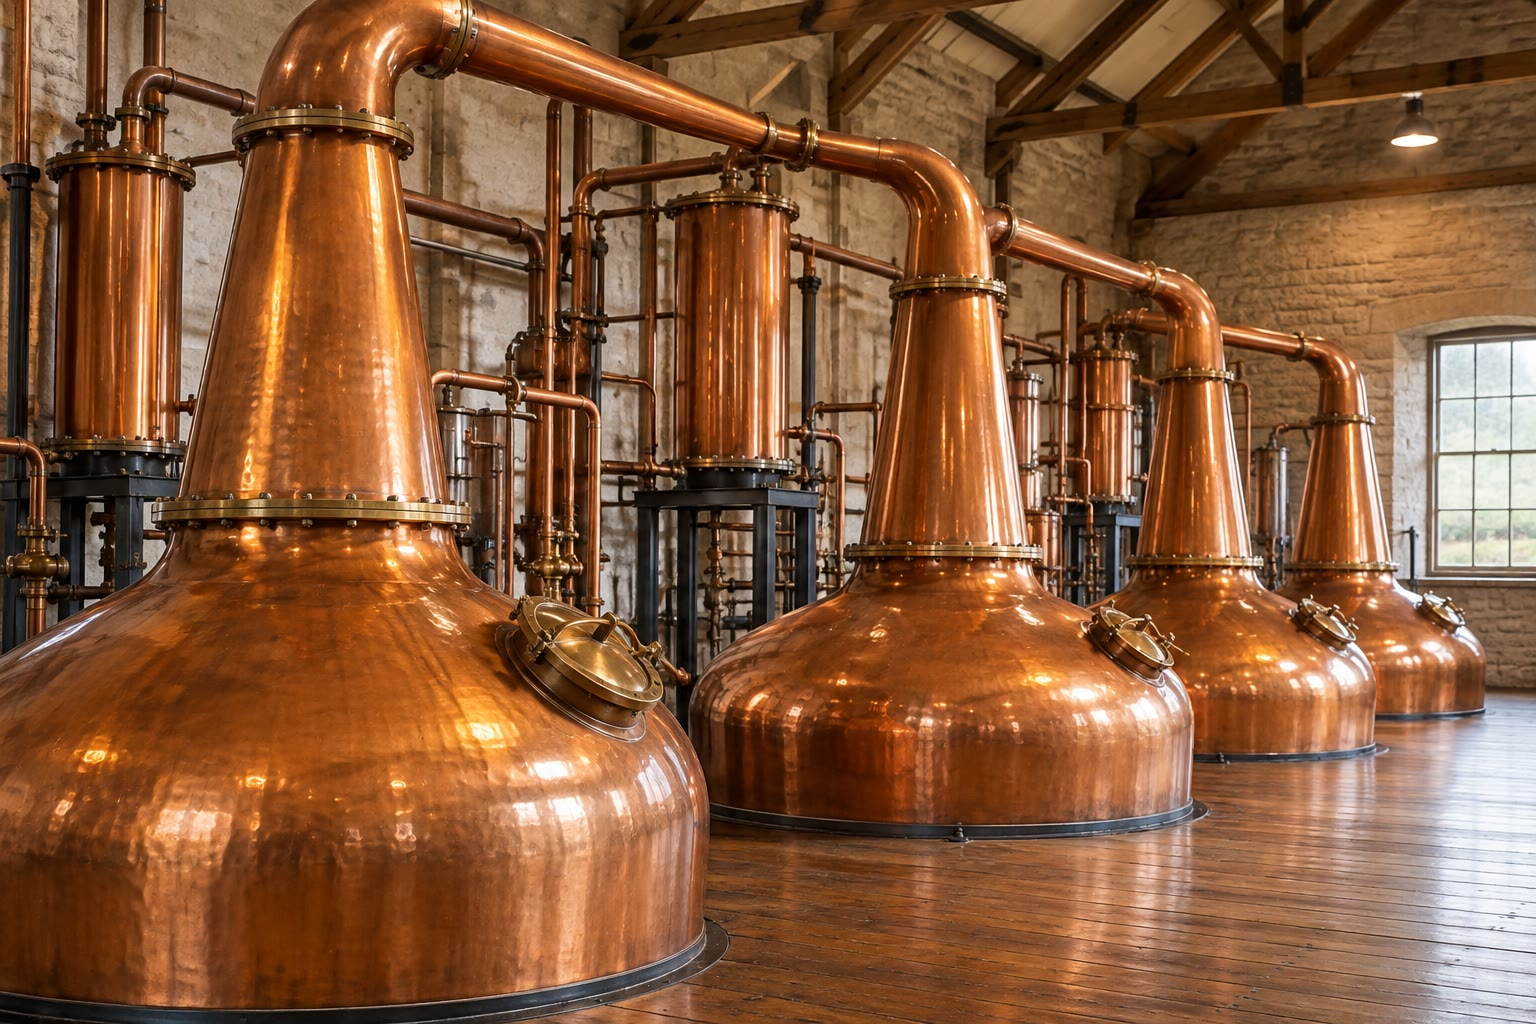
\includegraphics[width=0.62\linewidth]{images/book3/ai/b2-07-pot-stills.jpg}

{\small Koperen distilleerketels in een stokerij. Elke lading gefermenteerd beslag wordt
gekookt en de damp gecondenseerd: het eerste destillaat is verscheidene malen rijker
aan ethanol dan het beslag, en een tweede destillatie concentreert het verder.}
\end{omfigure}

\section{Ideale mengsels}

In dit hoofdstuk krijgen de twee vloeistoffen de nummers 1 (de vluchtigste, met het laagste
kookpunt) en 2; $x$ is de molfractie van 1 in de vloeistof, $y$ zijn
molfractie in de damp, die als ideaal gas behandeld wordt.

\begin{definition}[Binair diagram]\label{def:b2:liquid-vapour-diagrams:binary-diagram}
Een \emph{binair diagram}\index{binair diagram} toont voor een mengsel van twee
bestanddelen welke fasen aanwezig zijn en met welke samenstellingen, als
functie van de totale samenstelling en van één andere variabele. Een
\emph{isobaar diagram}\index{isobaar diagram} wordt getekend in het vlak
(samenstelling, temperatuur) bij vaste druk; een \emph{isotherm
diagram}\index{isotherm diagram} in het vlak (samenstelling, druk) bij
vaste temperatuur.
\end{definition}

\begin{definition}[Kookkromme en dauwkromme]\label{def:b2:liquid-vapour-diagrams:bubble-dew}
In een vloeistof-dampdiagram geeft de \emph{kookkromme}\index{kookkromme}
de samenstelling van de vloeistof in evenwicht met damp, de
\emph{dauwkromme}\index{dauwkromme} die van de damp in evenwicht met vloeistof. Voor een
mengsel met gegeven samenstelling bij vaste druk is het
\emph{beginkookpunt}\index{beginkookpunt} de temperatuur waarbij bij verwarmen de eerste dampbel
verschijnt, het \emph{dauwpunt}\index{dauwpunt} de
temperatuur waarbij bij afkoelen van de damp de eerste vloeistofdruppel verschijnt.
\end{definition}

\begin{proposition}[Ideale krommen]\label{prop:b2:liquid-vapour-diagrams:ideal-curves}
Voor een \omterm{def:b2:chemical-potential:ideal-mixture}{ideaal mengsel} bij temperatuur $T$, met $p_1^*$ en $p_2^*$ de dampdrukken
van de zuivere vloeistoffen, is de \omterm{def:b2:liquid-vapour-diagrams:bubble-dew}{kookkromme} van het \omterm{def:b2:liquid-vapour-diagrams:binary-diagram}{isotherme diagram}
de rechte $p = p_2^* + x(p_1^* - p_2^*)$, en is de \omterm{def:b2:liquid-vapour-diagrams:bubble-dew}{dauwkromme} de
hyperbool
\[
  p = \frac{1}{y/p_1^* + (1 - y)/p_2^*} .
\]
\end{proposition}

\begin{proof}
De \omterm{thm:b2:chemical-potential:raoult}{wet van Raoult} geeft de partiële drukken $p_1 = xp_1^*$ en $p_2 = (1 -
x)p_2^*$; hun som is de totale druk, lineair in $x$. In de damp is
$y = p_1/p$, dus $x = yp/p_1^*$ en $1 - x = (1 - y)p/p_2^*$; optellen geeft
$1 = p\,[y/p_1^* + (1 - y)/p_2^*]$.
\end{proof}

\begin{proposition}[De damp is rijker aan het vluchtigste bestanddeel]\label{prop:b2:liquid-vapour-diagrams:richer}
Voor een \omterm{def:b2:chemical-potential:ideal-mixture}{ideaal mengsel} met $p_1^* > p_2^*$ en $0 < x < 1$ is $y > x$.
\end{proposition}

\begin{proof}
$y = xp_1^*/p$ met $p = xp_1^* + (1 - x)p_2^* < p_1^*$, omdat $p$ een
gewogen gemiddelde is van $p_1^*$ en $p_2^*$, strikt ertussen. Dus $y >
x$.
\end{proof}

Het \omterm{def:b2:liquid-vapour-diagrams:binary-diagram}{isobare diagram} is het diagram dat een destillatie beschrijft, die bij
atmosferische druk verloopt. Er bestaat geen eenvoudige formule voor: voor elke temperatuur tussen
de twee kookpunten berekent men $p_1^*(T)$ en $p_2^*(T)$ (hier met de
vergelijking van Antoine, $\log_{10}(p^*/\unit{bar}) = A - B/(T + C)$, aangepast aan
gemeten dampdrukken), en daarna de samenstellingen van vloeistof en damp die
een totale druk van \qty{1.013}{bar} geven:
\[
  x = \frac{p - p_2^*(T)}{p_1^*(T) - p_2^*(T)}, \qquad y = \frac{x\,p_1^*(T)}{p} .
\]
De \omterm{def:b2:liquid-vapour-diagrams:bubble-dew}{kookkromme} is niet langer recht; de \omterm{def:b2:liquid-vapour-diagrams:bubble-dew}{dauwkromme} ligt er nog steeds boven, en
de damp is nog steeds rijker aan het lichte bestanddeel.

\begin{example}[Benzeen en tolueen bij \qty{90}{\degreeCelsius}]\label{ex:b2:liquid-vapour-diagrams:benzene-toluene}
Benzeen en tolueen vormen een bijna \omterm{def:b2:chemical-potential:ideal-mixture}{ideaal mengsel}. Bij \qty{90}{\degreeCelsius}
geven de vergelijkingen van Antoine $p_1^* = \qty{1.361}{bar}$ (benzeen) en $p_2^* =
\qty{0.542}{bar}$ (tolueen). Bij \qty{1.013}{bar}: $x = (1.013 - 0.542)/(1.361 -
0.542) = 0.575$ en $y = 0.575 \times 1.361/1.013 = 0.773$. Een vloeistof met 57.5~\%
benzeen (in mol) kookt bij \qty{90}{\degreeCelsius} en geeft een damp met
77~\%.
% ledger: antoine:benzene.A, antoine:benzene.B, antoine:benzene.C, antoine:toluene.A, antoine:toluene.B, antoine:toluene.C
\end{example}

\begin{omfigure}
\begin{tikzpicture}
\begin{axis}[omphase, width=0.47\linewidth, height=6cm, ymin=78, ymax=113,
  xlabel={$x$, $y$ (benzeen)}, ylabel={$T$ (\unit{\degreeCelsius})},
  title={\small isobaar, \qty{1.013}{bar}}]
\addplot[omliquidus] table[x=x, y=T] {figdata/out/bachelor-2-liquid-vapour-a.dat};
\addplot[omsolidus] table[x=y, y=T] {figdata/out/bachelor-2-liquid-vapour-a.dat};
\draw[tieline] (axis cs:0.405,95) -- (axis cs:0.626,95);
\fill (axis cs:0.5,95) circle (1.3pt);
\draw[->, thick] (axis cs:0.5,82) -- (axis cs:0.5,104) node[above, font=\scriptsize] {verwarmen};
\node[font=\scriptsize] at (axis cs:0.2,85) {vloeistof};
\node[font=\scriptsize] at (axis cs:0.85,108) {damp};
\node[font=\scriptsize, omDef, anchor=north] at (axis cs:0.22,96) {kookkromme};
\node[font=\scriptsize, omThm, anchor=south west] at (axis cs:0.62,101) {dauwkromme};
\end{axis}
\end{tikzpicture}\hfill
\begin{tikzpicture}
\begin{axis}[omphase, width=0.47\linewidth, height=6cm, ymin=0.3, ymax=1.1,
  xlabel={$x$, $y$ (benzeen)}, ylabel={$p$ (\unit{bar})},
  title={\small isotherm, \qty{80}{\degreeCelsius}}]
\addplot[omliquidus] table[x=x, y=pbub] {figdata/out/bachelor-2-liquid-vapour-b.dat};
\addplot[omsolidus] table[x=x, y=pdew] {figdata/out/bachelor-2-liquid-vapour-b.dat};
\node[font=\scriptsize] at (axis cs:0.75,0.98) {vloeistof};
\node[font=\scriptsize] at (axis cs:0.2,0.36) {damp};
\end{axis}
\end{tikzpicture}

{\small Benzeen--tolueen, berekend met de \omterm{thm:b2:chemical-potential:raoult}{wet van Raoult} en de vergelijkingen
van Antoine. Links, bij atmosferische druk: \omterm{def:b2:liquid-vapour-diagrams:bubble-dew}{kookkromme} (blauw) en \omterm{def:b2:liquid-vapour-diagrams:bubble-dew}{dauwkromme}
(rood); de vloeistof met samenstelling 0.5 begint te koken bij
\qty{92.1}{\degreeCelsius} en is volledig damp bij \qty{98.8}{\degreeCelsius}; bij
\qty{95}{\degreeCelsius} (gestreepte verbindingslijn) splitst ze in een vloeistof met 0.405
en een damp met 0.626. Rechts, bij \qty{80}{\degreeCelsius}: de \omterm{def:b2:liquid-vapour-diagrams:bubble-dew}{kookkromme} is
recht, de \omterm{def:b2:liquid-vapour-diagrams:bubble-dew}{dauwkromme} een hyperbool, en de vloeistof ligt nu bovenaan.}
% ledger: antoine:benzene.A, antoine:toluene.A (all six parameters in figdata/bachelor-2/liquid-vapour.py)
\end{omfigure}

\section{Een diagram lezen}

\begin{proposition}[Variantie van een binair tweefasensysteem]\label{prop:b2:liquid-vapour-diagrams:variance}
Een mengsel van twee bestanddelen in twee fasen heeft \omterm{def:b2:equilibrium-shifts:variance}{variantie} 2. Bij vaste druk
legt de temperatuur alleen de samenstellingen van beide fasen vast: ze worden afgelezen
aan de uiteinden van het horizontale lijnstuk door het representatieve punt,
de verbindingslijn genoemd.
\end{proposition}

\begin{proof}
Intensieve variabelen: $T$, $p$, $x$, $y$. Betrekkingen: gelijkheid van de \omterm{def:b2:chemical-potential:chemical-potential}{chemische
potentialen} van 1 en van 2 tussen de fasen. $v = 4 - 2 = 2$ (de faseregel
$v = n - r + 2 - \varphi$ geeft hetzelfde met $n = 2$, $r = 0$, $\varphi = 2$).
Een vaste $p$ laat één vrijheidsgraad over: $x(T)$ en $y(T)$ zijn de twee krommen.
\end{proof}

\begin{theorem}[Hefboomregel]\label{thm:b2:liquid-vapour-diagrams:lever}
Een mengsel met totale samenstelling $z$, gesplitst in een vloeistof met samenstelling $x$
en een damp met samenstelling $y$, bevat hoeveelheden $n_L$ vloeistof en $n_V$
damp zodat
\[
  n_L\,(z - x) = n_V\,(y - z), \qquad \frac{n_V}{n_L + n_V} = \frac{z - x}{y - x} .
\]
Dit is de \emph{hefboomregel}\index{hefboomregel}: elke fase is des te
overvloediger naarmate haar samenstelling dichter bij de totale ligt, zoals de gewichten aan
een hefboom die om $z$ draait.
\end{theorem}

\begin{proof}
Behoud van bestanddeel 1: $(n_L + n_V)z = n_Lx + n_Vy$, dus $n_L(z - x) =
n_V(y - z)$; deel door $n_L + n_V$ en herschik.
\end{proof}

De \omterm{thm:b2:liquid-vapour-diagrams:lever}{hefboomregel} geldt met molfracties en hoeveelheden, zoals hier, of met massafracties
en massa's: het gebruikte behoud is hetzelfde.

\begin{method}[Een binair diagram lezen]\label{met:b2:liquid-vapour-diagrams:read-diagram}
\begin{enumerate}
  \item Zet het punt (totale samenstelling, temperatuur) uit en benoem zijn
        gebied: vloeistof, damp, of vloeistof + damp.
  \item Teken in een tweefasengebied de verbindingslijn door het punt; haar uiteinden
        geven de samenstellingen van de vloeistof (op de \omterm{def:b2:liquid-vapour-diagrams:bubble-dew}{kookkromme}) en van de
        damp (op de \omterm{def:b2:liquid-vapour-diagrams:bubble-dew}{dauwkromme}).
  \item Haal de verhoudingen van de fasen uit de \omterm{thm:b2:liquid-vapour-diagrams:lever}{hefboomregel}.
  \item Om een verwarming te volgen, schuif je het punt omhoog: de eerste bel verschijnt
        op de \omterm{def:b2:liquid-vapour-diagrams:bubble-dew}{kookkromme}, de laatste druppel verdwijnt op de \omterm{def:b2:liquid-vapour-diagrams:bubble-dew}{dauwkromme};
        daartussen wordt de vloeistof armer aan het lichte bestanddeel.
\end{enumerate}
\end{method}

\begin{example}[Een flash bij \qty{95}{\degreeCelsius}]\label{ex:b2:liquid-vapour-diagrams:flash}
\qty{100}{mol} van een equimolair mengsel benzeen--tolueen wordt bij atmosferische druk op
\qty{95}{\degreeCelsius} gebracht. De verbindingslijn geeft $x =
0.405$, $y = 0.626$; de dampfractie is $(0.500 - 0.405)/(0.626 - 0.405) =
0.43$: \qty{43}{mol} damp met $43 \times 0.626 = \qty{27}{mol}$
benzeen, \qty{57}{mol} vloeistof met \qty{23}{mol}. Eén evenwichtstrap
verrijkt, maar slechts een beetje.
\end{example}

\section{Reële mengsels en azeotropen}

Wanneer de \omterm{def:b2:chemical-potential:activity-coefficient}{activiteitscoëfficiënten} niet gelijk zijn aan 1 (\cref{ch:b2:chemical-potential}),
wijken de partiële drukken af van de rechte lijnen van Raoult. Bij een positieve
afwijking ($\gamma > 1$: ongelijke moleculen trekken elkaar minder aan dan gelijke)
ligt de totale druk boven de ideale lijn; bij een negatieve afwijking
eronder. Is de afwijking sterk genoeg, dan gaat de totale druk door een
extremum.

\begin{definition}[Azeotroop]\label{def:b2:liquid-vapour-diagrams:azeotrope}
Een \emph{azeotroop}\index{azeotroop} is een vloeibaar mengsel dat kookt zonder
van samenstelling te veranderen: de damp die het geeft, heeft zijn eigen samenstelling. Een
\emph{positieve azeotroop}\index{positieve azeotroop} (positieve afwijking) heeft
een drukmaximum in het \omterm{def:b2:liquid-vapour-diagrams:binary-diagram}{isotherme diagram} en een minimum van de kooktemperatuur
in het \omterm{def:b2:liquid-vapour-diagrams:binary-diagram}{isobare diagram}; een \emph{negatieve azeotroop}\index{negatieve azeotroop}
het omgekeerde.
\end{definition}

\begin{theorem}[Gibbs--Konovalov]\label{thm:b2:liquid-vapour-diagrams:konovalov}
In een binair vloeistof-dampdiagram hebben bij een extremum van de totale druk (bij
vaste temperatuur) of van de kooktemperatuur (bij vaste druk) de
vloeistof en de damp dezelfde samenstelling. Omgekeerd hebben de krommen, waar de
twee samenstellingen gelijk zijn, een gemeenschappelijke horizontale raaklijn.
\end{theorem}

\begin{proof}[Bewijs bij vaste temperatuur]
De betrekking van Gibbs--Duhem voor de vloeistof bij vaste $T$ (het kleine effect van $p$
op de vloeistof verwaarloosd) is $x\,d\mu_1 + (1 - x)\,d\mu_2 = 0$. In evenwicht is
$\mu_i = \mu_i^\circ + RT\ln(p_i/p^\circ)$ met $p_1 = yp$, $p_2 = (1 - y)p$, dus
\[
  x\,d\ln(yp) + (1 - x)\,d\ln((1 - y)p) = 0
  \quad\Longrightarrow\quad
  d\ln p = -\Big(\frac{x}{y} - \frac{1 - x}{1 - y}\Big)dy
  = \frac{y - x}{y(1 - y)}\,dy .
\]
Omdat $y$ toeneemt met $x$ (anders zou de vloeistof instabiel zijn), is
$dp/dx = 0$ precies waar $y = x$. Het isobare geval volgt uit een gelijkaardige
berekening die de temperatuurafhankelijkheid van de $\mu_i^\circ$ behoudt; ze wordt
hier niet uitgevoerd.
\end{proof}

De formule zegt meer: waar $y > x$, neemt de druk toe met $x$ ---
het bestanddeel toevoegen dat in de damp verrijkt wordt, maakt de vloeistof
vluchtiger, wat de eerste wet van Konovalov is.

\begin{example}[Ethanol en water]\label{ex:b2:liquid-vapour-diagrams:ethanol-water}
Ethanol en water wijken positief af van de \omterm{thm:b2:chemical-potential:raoult}{wet van Raoult} en vormen een \omterm{def:b2:liquid-vapour-diagrams:azeotrope}{azeotroop}
met 95~\% ethanol in massa bij atmosferische druk. Met $M = 46.07$ en
\qty{18.02}{g/mol} is de molfractie ethanol ervan
\[
  x_{\text{az}} = \frac{95/46.07}{95/46.07 + 5/18.02} = 0.881 .
\]
Hij kookt iets onder zuivere ethanol (\qty{78.3}{\degreeCelsius}). Het diagram
hieronder is berekend met een activiteitsmodel met één parameter, $\ln\gamma_1 = A(1 -
x)^2$, $\ln\gamma_2 = Ax^2$, waarvan de parameter ($A = 1.09$) zo aangepast is dat de
\omterm{def:b2:liquid-vapour-diagrams:azeotrope}{azeotroop} bij die samenstelling valt: het model geeft de vorm goed weer, en
plaatst de \omterm{def:b2:liquid-vapour-diagrams:azeotrope}{azeotroop} bij \qty{77.9}{\degreeCelsius}.
% ledger: azeo:ethanol-water.w, aw:C, aw:H, aw:O, antoine:ethanol.A, antoine:ethanol.B, antoine:ethanol.C, antoine:water.A, antoine:water.B, antoine:water.C
\end{example}

\begin{omfigure}
\begin{tikzpicture}
\begin{axis}[omphase, width=0.47\linewidth, height=6cm, ymin=76, ymax=101,
  xlabel={$x$, $y$ (ethanol)}, ylabel={$T$ (\unit{\degreeCelsius})},
  title={\small ethanol--water (model)}]
\addplot[omliquidus] table[x=x, y=T] {figdata/out/bachelor-2-liquid-vapour-c.dat};
\addplot[omsolidus] table[x=y, y=T] {figdata/out/bachelor-2-liquid-vapour-c.dat};
\fill (axis cs:0.881,77.92) circle (1.5pt);
\draw[densely dotted] (axis cs:0.881,77.92) -- (axis cs:0.881,76);
\node[font=\scriptsize, anchor=south] at (axis cs:0.80,80.5) {azeotroop};
\draw[thin] (axis cs:0.80,80.5) -- (axis cs:0.875,78.2);
\node[font=\scriptsize] at (axis cs:0.25,79.5) {vloeistof};
\node[font=\scriptsize] at (axis cs:0.5,95) {damp};
\end{axis}
\end{tikzpicture}\hfill
\begin{tikzpicture}
\begin{axis}[omphase, width=0.47\linewidth, height=6cm, ymin=78, ymax=120,
  xlabel={$x$, $y$ (bestanddeel 1)}, ylabel={$T$ (\unit{\degreeCelsius})},
  title={\small negatieve afwijking (model)}]
\addplot[omliquidus] table[x=x, y=T] {figdata/out/bachelor-2-liquid-vapour-d.dat};
\addplot[omsolidus] table[x=y, y=T] {figdata/out/bachelor-2-liquid-vapour-d.dat};
\fill (axis cs:0.29,116.7) circle (1.5pt);
\node[font=\scriptsize, anchor=west] at (axis cs:0.33,118) {azeotroop};
\node[font=\scriptsize] at (axis cs:0.6,85) {vloeistof};
\node[font=\scriptsize] at (axis cs:0.75,116) {damp};
\end{axis}
\end{tikzpicture}

{\small Links: ethanol--water bij atmosferische druk, volgens een model met één parameter,
aangepast aan de samenstelling van de \omterm{def:b2:liquid-vapour-diagrams:azeotrope}{azeotroop} (0.881); de \omterm{def:b2:liquid-vapour-diagrams:azeotrope}{azeotroop} kookt onder
beide zuivere vloeistoffen. Rechts: een modelpaar met een sterke negatieve afwijking
($A = -2.0$, dampdrukken van benzeen en tolueen); de \omterm{def:b2:liquid-vapour-diagrams:azeotrope}{azeotroop} kookt
boven beide.}
% ledger: azeo:ethanol-water.w, antoine:ethanol.A, antoine:water.A (model in figdata/bachelor-2/liquid-vapour.py)
\end{omfigure}

\section{Gefractioneerde destillatie}

\begin{definition}[Gefractioneerde destillatie]\label{def:b2:liquid-vapour-diagrams:fractional-distillation}
\emph{Gefractioneerde destillatie}\index{gefractioneerde destillatie} scheidt de
bestanddelen van een vloeibaar mengsel in een kolom waarin een opstijgende damp en een
neerdalende vloeistof herhaaldelijk met elkaar in contact gebracht worden. Een \emph{theoretische
schotel}\index{theoretische schotel} is een trap van de kolom waarvan de vertrekkende damp
en vloeistof met elkaar in evenwicht zijn. De
\emph{refluxverhouding}\index{refluxverhouding} is de verhouding van de hoeveelheid condensaat die
naar de top van de kolom teruggaat, tot de hoeveelheid die als destillaat wordt afgetapt.
\end{definition}

Op elke schotel borrelt de damp van beneden door de vloeistof van boven; hij
vertrekt rijker aan het lichte bestanddeel, de vloeistof armer. Bovenaan wordt de damp
gecondenseerd, een deel teruggestuurd als reflux, de rest afgetapt als het
destillaat; onderaan kookt een verdamper een deel van de vloeistof. Bij
\textit{totale reflux} wordt niets afgetapt: de kolom werkt dan op haar best,
en de damp die een schotel verlaat, heeft de samenstelling van de vloeistof die erop
neerdaalt.


Voor een ideaal paar verandert de \textit{relatieve vluchtigheid} $\alpha = p_1^*/p_2^*$
weinig over de kolom: van 2.60 bij het kookpunt van benzeen tot
2.35 bij dat van tolueen. Op elke \omterm{def:b2:liquid-vapour-diagrams:fractional-distillation}{theoretische schotel} geldt
\[
  \frac{y}{1 - y} = \frac{xp_1^*}{(1 - x)p_2^*} = \alpha\,\frac{x}{1 - x} .
\]

\begin{omfigure}
\begin{minipage}[b]{0.58\linewidth}\centering
\begin{tikzpicture}[font=\small, >={Stealth}, scale=0.8, every node/.style={transform shape}]
  \draw[thick, fill=gray!8] (0,0) rectangle (1.8,7);
  \foreach \k in {1,...,6} {
    \pgfmathsetmacro{\yy}{\k}
    \ifodd\k
      \draw[thick] (0,\yy) -- (1.45,\yy); \draw[thick] (1.45,\yy) -- (1.45,\yy-0.55);
    \else
      \draw[thick] (0.35,\yy) -- (1.8,\yy); \draw[thick] (0.35,\yy) -- (0.35,\yy-0.55);
    \fi
    \fill[omDef!25] (0.02,\yy) rectangle (1.78,\yy+0.12);
  }
  \foreach \k in {1,...,6} \node[font=\scriptsize, anchor=east] at (-0.1,\k) {schotel \k};
  \draw[->, thick, omThm] (0.9,7.0) -- (0.9,7.9) -- (2.8,7.9);
  \draw[thick, fill=white] (2.8,7.6) rectangle (3.6,8.2);
  \node[anchor=west, font=\scriptsize] at (3.65,7.9) {condensor};
  \draw[->, thick, omDef] (3.2,7.6) -- (3.2,5.6);
  \draw[thick, fill=omDef!20] (2.7,5.0) rectangle (3.7,5.6);
  \node[font=\scriptsize, anchor=west] at (3.75,5.3) {refluxvat};
  \draw[->, thick, omDef] (2.7,5.3) -- (2.1,5.3) -- (2.1,6.6) -- (1.8,6.6);
  \node[font=\scriptsize, anchor=west, omDef] at (2.15,6.1) {reflux};
  \draw[->, thick, omDef] (3.2,5.0) -- (3.2,4.4) -- (4.4,4.4) node[right] {destillaat};
  \draw[->, thick] (-2.2,3.5) -- (0,3.5) node[pos=0, left] {voeding};
  \draw[thick, fill=omDef!20] (0.2,-1.3) rectangle (1.6,-0.6);
  \node[font=\scriptsize] at (0.9,-0.95) {verdamper};
  \draw[thick, omDef] (0.9,0) -- (0.9,-0.6);
  \draw[->, thick, omThm] (1.6,-0.8) -- (2.1,-0.8) -- (2.1,0.4) -- (1.8,0.4);
  \draw[->, thick, omDef] (0.9,-1.3) -- (0.9,-1.8) -- (2.6,-1.8) node[right] {bodemproduct};
  \draw[->, omThm, thick] (2.6,1.5) -- (2.6,3.0) node[midway, right, font=\scriptsize, align=left] {damp\\ stijgt};
  \draw[->, omDef, thick] (-1.4,5.8) -- (-1.4,4.3) node[midway, left, font=\scriptsize, align=right] {vloeistof\\ daalt};
\end{tikzpicture}
\end{minipage}\hfill
\begin{minipage}[b]{0.34\linewidth}\centering
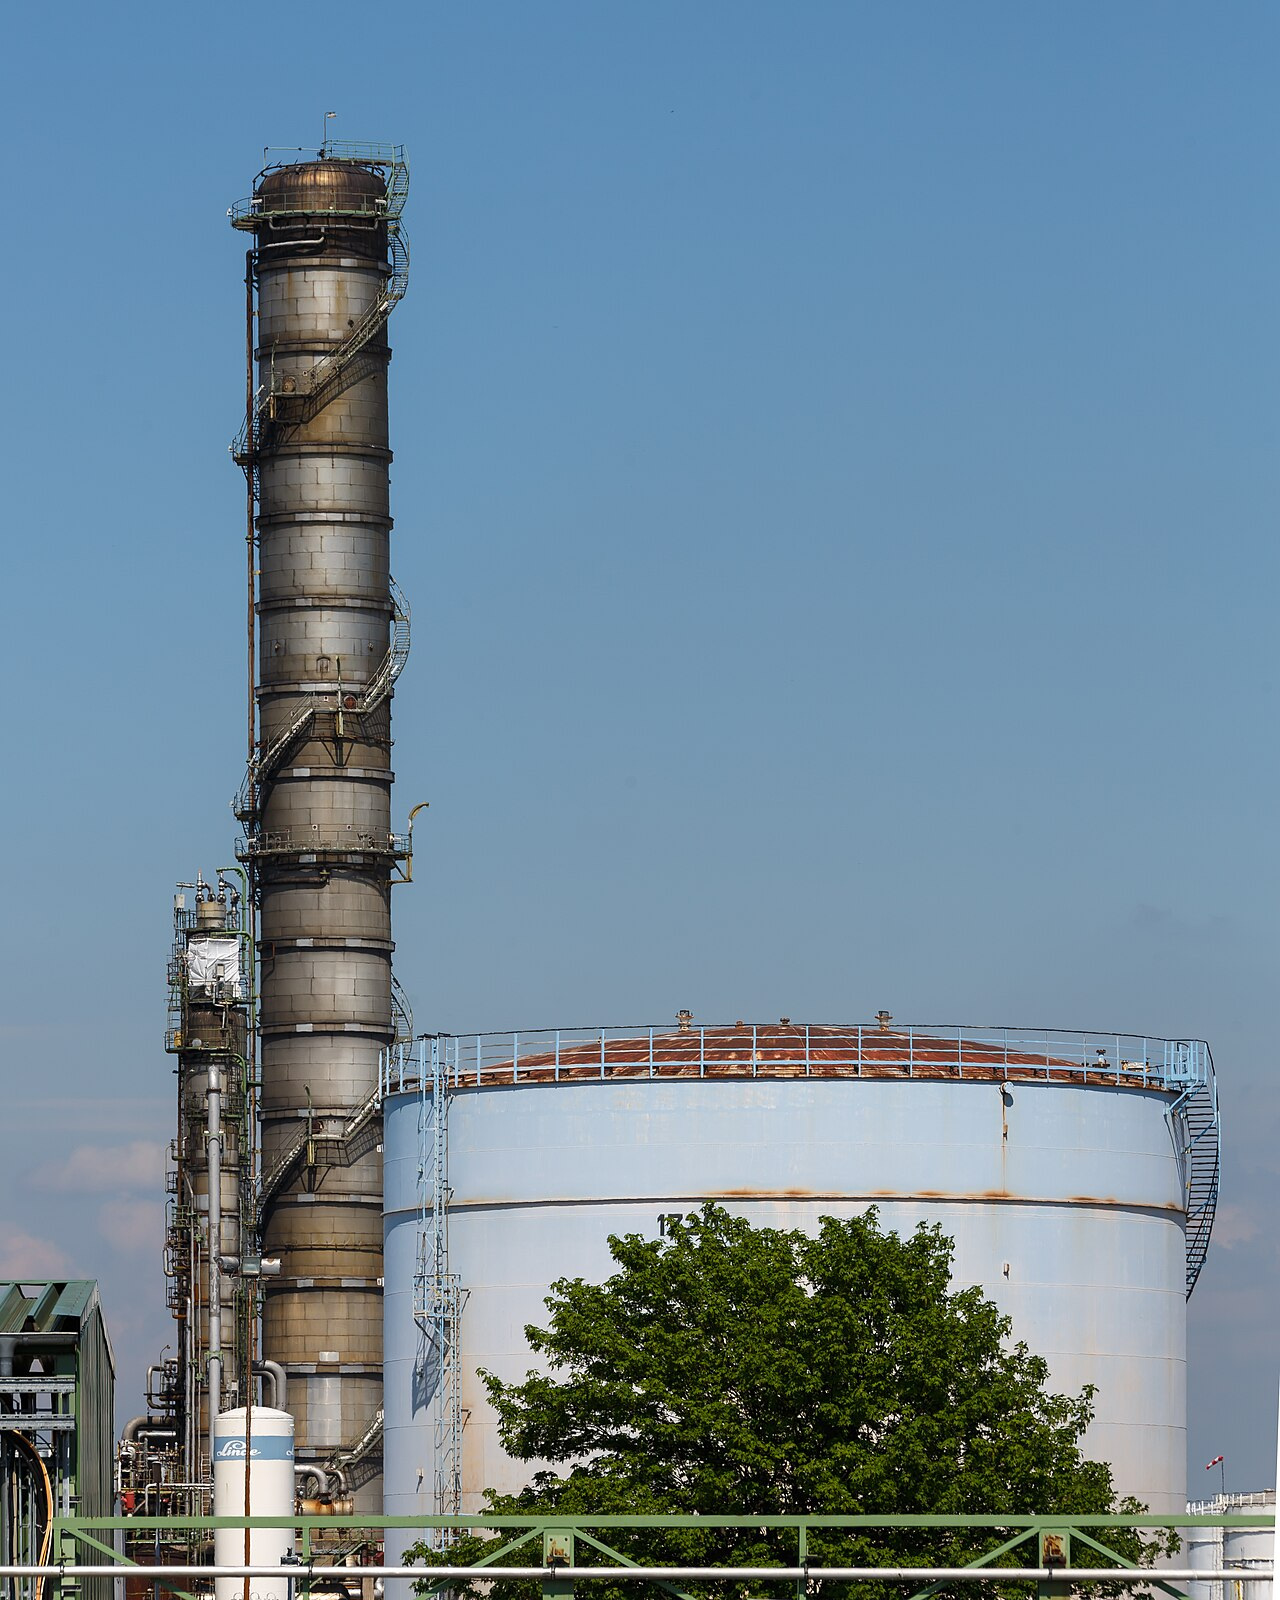
\includegraphics[width=\linewidth]{images/book3/refinery-column.jpg}
\end{minipage}

{\small Links: een schotelkolom. De vloeistof stroomt over elke schotel en via de
valpijp naar de schotel eronder; de damp stijgt door de schotels en borrelt
door de vloeistof. De gecondenseerde damp wordt gedeeltelijk teruggestuurd als reflux; de
verdamper onderaan levert de damp. Rechts: een destillatiekolom van een
raffinaderij (Keulen, 2014), die tientallen schotels bevat. (Foto: CEphoto,
Uwe Aranas, CC BY-SA 3.0, Wikimedia Commons.)}
\end{omfigure}

\begin{proposition}[Fenske]\label{prop:b2:liquid-vapour-diagrams:fenske}
Bij totale reflux, met een constante relatieve vluchtigheid $\alpha$, is het aantal
\omterm{def:b2:liquid-vapour-diagrams:fractional-distillation}{theoretische schotels} dat nodig is om van een bodemvloeistof $x_B$ naar een destillaat
$x_D$ te gaan, minstens
\[
  N_{\min} = \frac{1}{\ln\alpha}\,\ln\!\left[\frac{x_D}{1 - x_D}\cdot\frac{1 - x_B}{x_B}\right] .
\]
\end{proposition}

\begin{proof}
Nummer de schotels van onderen, met de verdamper als schotel 1. Bij totale reflux
heeft de vloeistof die op schotel $k + 1$ neerdaalt, de samenstelling van de damp
die schotel $k$ verlaat: $x_{k+1} = y_k$. Met $r = x/(1 - x)$ geeft elke schotel
$r(y_k) = \alpha\,r(x_k)$, dus $r(x_{k+1}) = \alpha\,r(x_k)$, en na $N$
schotels heeft de gecondenseerde damp $r(x_D) = \alpha^N r(x_B)$. Logaritmen nemen
geeft $N$. Met een eindige reflux is de neerdalende vloeistof armer dan de
opstijgende damp, verrijkt elke schotel minder, en zijn er meer schotels nodig.
\end{proof}

In het $(x, y)$-diagram is dezelfde constructie een trap tussen de
evenwichtskromme en de diagonaal $y = x$: elke trede is één \omterm{def:b2:liquid-vapour-diagrams:fractional-distillation}{theoretische
schotel}.

\begin{omfigure}
\begin{tikzpicture}
\begin{axis}[width=0.55\linewidth, height=0.55\linewidth, xmin=0, xmax=1,
  ymin=0, ymax=1, axis x line=bottom, axis y line=left,
  xlabel={$x$ (benzeen, vloeistof)}, ylabel={$y$ (benzeen, damp)},
  tick label style={font=\small}, label style={font=\small}]
\addplot[omThm, thick] table[x=x, y=y] {figdata/out/bachelor-2-liquid-vapour-f-eq.dat};
\addplot[black!50] coordinates {(0,0) (1,1)};
\addplot[omDef, thick] table[x=x, y=y] {figdata/out/bachelor-2-liquid-vapour-f.dat};
\draw[densely dotted] (axis cs:0.95,0) -- (axis cs:0.95,0.95);
\draw[densely dotted] (axis cs:0.05,0) -- (axis cs:0.05,0.05);
\node[font=\scriptsize, anchor=south east] at (axis cs:0.945,0.02) {$x_D$};
\node[font=\scriptsize, anchor=south west] at (axis cs:0.05,0.02) {$x_B$};
\end{axis}
\end{tikzpicture}

{\small Schotels bij totale reflux voor benzeen--tolueen, vanaf een destillaat van
0.95 naar beneden: elke horizontale trede gaat van een damp naar de vloeistof in
evenwicht ermee (één schotel), elke verticale trede van die vloeistof naar de
damp van de schotel eronder. Zeven treden brengen de vloeistof onder $x_B = 0.05$;
de formule van Fenske geeft 6.5.}
% ledger: antoine:benzene.A, antoine:toluene.A (computed in figdata/bachelor-2/liquid-vapour.py)
\end{omfigure}

\begin{proposition}[Een kolom kan een azeotroop niet oversteken]\label{prop:b2:liquid-vapour-diagrams:azeotrope-limit}
In een mengsel met een \omterm{def:b2:liquid-vapour-diagrams:azeotrope}{azeotroop} levert een kolom die aan één kant van de azeotrope
samenstelling gevoed wordt, op zijn best de \omterm{def:b2:liquid-vapour-diagrams:azeotrope}{azeotroop} aan het ene uiteinde en het zuivere bestanddeel
van die kant aan het andere.
\end{proposition}

\begin{proof}
Bij de \omterm{def:b2:liquid-vapour-diagrams:azeotrope}{azeotroop} raakt de evenwichtskromme de diagonaal: $y = x$. Dichtbij
wordt elke trede van de trap verdwijnend klein, zodat geen eindig aantal
schotels haar bereikt, en geen enkele haar oversteekt.
\end{proof}

\begin{method}[Een gefractioneerde destillatie voorspellen]\label{met:b2:liquid-vapour-diagrams:predict-distillation}
\begin{enumerate}
  \item Zoek in het \omterm{def:b2:liquid-vapour-diagrams:binary-diagram}{isobare diagram} het laagste kookpunt dat vanuit de voeding bereikbaar is:
        een zuiver bestanddeel of een \omterm{def:b2:liquid-vapour-diagrams:azeotrope}{positieve azeotroop}. Dat komt
        bovenaan uit.
  \item Het hoogste kookpunt aan dezelfde kant (zuiver bestanddeel of
        \omterm{def:b2:liquid-vapour-diagrams:azeotrope}{negatieve azeotroop}) blijft in de ketel.
  \item Kijk bij een \omterm{def:b2:liquid-vapour-diagrams:azeotrope}{azeotroop} aan welke kant ervan de voeding ligt: alleen het zuivere
        bestanddeel van die kant kan verkregen worden.
  \item Gebruik voor het aantal schotels de formule van Fenske of de trap,
        en tel er schotels bij voor de eindige reflux die werkelijk gebruikt wordt.
\end{enumerate}
\end{method}

Voor ethanol en water, gevoed onder 0.881, levert de top op zijn best de
\omterm{def:b2:liquid-vapour-diagrams:azeotrope}{azeotroop} en de bodem water: geen enkele kolom geeft absolute ethanol. Het drogen van
het laatste procent vereist een andere methode --- een moleculaire zeef die water adsorbeert, of
een derde bestanddeel dat toegevoegd wordt om de \omterm{def:b2:liquid-vapour-diagrams:azeotrope}{azeotroop} te breken.

\begin{omfigure}
\begin{tikzpicture}[font=\small, scale=0.95, >={Stealth}]
  \pic[transform shape] at (0,0) {heatingmantle};
  \pic[transform shape] at (0,0) {rbflask={0.45}{orange!25}};
  \foreach \x/\y in {-0.35/0.25,0.05/0.18,0.35/0.3}
    \fill[black!55] (\x,\y) circle (0.06);
  % Vigreux column from the flask neck (0,3) to (0,6)
  \draw[om glass] (-0.22,3.0) -- (-0.22,6.0) (0.22,3.0) -- (0.22,6.0);
  \foreach \yy in {3.4,3.9,4.4,4.9,5.4} {
    \draw[om glass] (-0.22,\yy) -- (-0.06,\yy+0.18) -- (-0.22,\yy+0.3);
    \draw[om glass] (0.22,\yy+0.15) -- (0.06,\yy+0.33) -- (0.22,\yy+0.45);
  }
  \pic[transform shape] (s) at (0,6.0) {stillhead};
  \pic[transform shape] at ($(s-top)+(0,-0.75)$) {thermometer};
  \pic[transform shape, rotate=-20] (c) at (s-arm) {liebig={3.4}};
  % ground-glass joint between the head's side arm and the condenser
  \draw[om glass, fill=white, rotate around={-20:(s-arm)}] ($(s-arm)+(-0.12,-0.17)$) rectangle ($(s-arm)+(0.14,0.17)$);
  \coordinate (cend) at ($(s-arm)+(-20:3.4)$);
  \pic[transform shape] (a) at (cend) {adapter};
  \pic[transform shape] at ($(a-tip)+(0,-2.4)$) {erlenmeyer={0.22}{orange!12}};
  \draw[<-, omProp, thick] (-0.25,4.6) -- (-1.6,4.6) node[left, text=black,
    align=right] {vigreuxkolom\\ (inkepingen vermenigvuldigen\\ de contacten)};
  \draw[<-, omProp, thick] (0.12,6.72) -- (-1.4,7.4) node[left, text=black,
    align=right] {thermometerbol\\ ter hoogte van de zijarm};
  \draw[<-, omProp, thick] (1.08,0.3) -- (2.3,-0.2) node[right, text=black]
    {verwarmingsmantel};
  \draw[<-, omProp, thick] ($(a-tip)+(0.75,-2.0)$) -- ++(1.0,0.2)
    node[right, text=black] {destillaat};
\end{tikzpicture}

{\small \omterm{def:b2:liquid-vapour-diagrams:fractional-distillation}{Gefractioneerde destillatie} in het laboratorium. Een vigreuxkolom tussen
de kolf en de destillatiekop speelt de rol van enkele \omterm{def:b2:liquid-vapour-diagrams:fractional-distillation}{theoretische schotels}: damp
condenseert op de inkepingen en verdampt opnieuw op weg naar boven. De
temperatuur aan de kop blijft op het kookpunt van het vluchtigste
bestanddeel zolang dat overdestilleert, en stijgt dan.}
\end{omfigure}

\begin{inthelab}[Twee vloeistoffen scheiden door gefractioneerde destillatie]
De kolf wordt hoogstens half gevuld, met kookstenen, en zacht verwarmd
zodat de ring van condenserende damp langzaam in de kolom klimt: een kolom
die door te snel verwarmen overstroomt, verliest haar schotels. De koptemperatuur wordt om de
paar milliliter genoteerd; de opvangkolf wordt gewisseld wanneer ze begint te stijgen (bij elke
temperatuurtrap wordt een \textit{fractie} opgevangen), en het verwarmen wordt
gestopt voordat de kolf droogkookt.
\end{inthelab}

\section{Gedeeltelijk mengbare en niet-mengbare vloeistoffen}

\begin{definition}[Ontmengingsgebied]\label{def:b2:liquid-vapour-diagrams:miscibility-gap}
Een \emph{ontmengingsgebied}\index{ontmengingsgebied} is het gebied van totale
samenstellingen waarover twee vloeistoffen, bij een gegeven temperatuur, uiteenvallen in twee
vloeistoflagen, elk verzadigd met het andere bestanddeel. Een
\emph{heteroazeotroop}\index{heteroazeotroop} is het kookpunt van zo'n
vloeistof met twee lagen: de twee vloeistoflagen en de damp bestaan naast elkaar bij een vaste
temperatuur en met een vaste dampsamenstelling.
\end{definition}

Bij de \omterm{def:b2:liquid-vapour-diagrams:miscibility-gap}{heteroazeotroop} zijn twee bestanddelen verdeeld over drie fasen: bij vaste
druk is de \omterm{def:b2:equilibrium-shifts:variance}{variantie} $2 + 2 - 3 - 1 = 0$. De temperatuur blijft
constant, zoals bij het kookpunt van een zuivere vloeistof, zolang beide lagen
aanwezig zijn.

\begin{omfigure}
\begin{tikzpicture}[font=\small, x=6cm, y=0.08cm]
  \draw[->] (0,0) -- (1.05,0) node[right] {$x$};
  \draw[->] (0,0) -- (0,62) node[above] {$T$};
  \node[below] at (0,0) {2}; \node[below] at (1,0) {1};
  % boiling points: 2 at 50, 1 at 42; heteroazeotrope at 25 with layers 0.1 and 0.85, vapour 0.6
  \draw[omliquidus] (0,50) .. controls (0.04,38) and (0.08,30) .. (0.1,25);
  \draw[omliquidus] (1,42) .. controls (0.95,34) and (0.9,28) .. (0.85,25);
  \draw[omsolidus] (0,50) .. controls (0.25,46) and (0.5,35) .. (0.6,25);
  \draw[omsolidus] (1,42) .. controls (0.9,37) and (0.7,30) .. (0.6,25);
  \draw[thick] (0.1,25) -- (0.85,25);
  \draw[omliquidus] (0.1,25) -- (0.07,2);
  \draw[omliquidus] (0.85,25) -- (0.9,2);
  \fill (0.6,25) circle[radius=2pt];
  \node[font=\scriptsize] at (0.47,6) {twee vloeistoflagen};
  \node[font=\scriptsize] at (0.5,55) {damp};
  \node[font=\scriptsize] at (0.035,12) {L$_2$};
  \node[font=\scriptsize] at (0.96,12) {L$_1$};
  \node[font=\scriptsize, align=center] at (0.3,33) {L$_2$ + V};
  \node[font=\scriptsize, anchor=west] at (1.06,36) {L$_1$ + V};
  \draw[thin] (1.06,36) -- (0.86,29.5);
  \node[font=\scriptsize, anchor=north] at (0.6,24) {heteroazeotroop};
\end{tikzpicture}

{\small Schematisch \omterm{def:b2:liquid-vapour-diagrams:binary-diagram}{isobaar diagram} van twee gedeeltelijk mengbare vloeistoffen. Onder de
temperatuur van de \omterm{def:b2:liquid-vapour-diagrams:miscibility-gap}{heteroazeotroop} splitst de vloeistof over een breed gebied van
samenstellingen in twee lagen L$_1$ en
L$_2$ (het \omterm{def:b2:liquid-vapour-diagrams:miscibility-gap}{ontmengingsgebied}); op de
horizontale lijn koken de twee lagen samen tot een damp met vaste
samenstelling (punt).}
\end{omfigure}

\begin{definition}[Stoomdestillatie]\label{def:b2:liquid-vapour-diagrams:steam-distillation}
\emph{Stoomdestillatie}\index{stoomdestillatie} is de destillatie van een
vloeistof die niet mengbaar is met water, door er stoom doorheen te blazen: het mengsel kookt
onder het kookpunt van beide vloeistoffen, en het destillaat scheidt zich in
twee lagen.
\end{definition}

\omterm{def:b2:liquid-vapour-diagrams:steam-distillation}{Stoomdestillatie} verschilt van de hydrodestillatie van het schoolboek
alleen in de manier waarop het water wordt aangevoerd: stoom die door het materiaal geblazen wordt, in plaats
van materiaal dat in water gekookt wordt. De thermodynamica is dezelfde.

\begin{proposition}[Koken van twee niet-mengbare vloeistoffen]\label{prop:b2:liquid-vapour-diagrams:steam}
Twee niet-mengbare vloeistoffen die met elkaar in contact zijn, koken bij de temperatuur waarbij de som van
hun dampdrukken gelijk is aan de uitwendige druk, $p_1^*(T) + p_2^*(T) =
p$, lager dan beide kookpunten. Het destillaat bevat de twee vloeistoffen
in de massaverhouding
\[
  \frac{m_1}{m_2} = \frac{p_1^*\,M_1}{p_2^*\,M_2} .
\]
\end{proposition}

\begin{proof}
Elke zuivere vloeistof oefent haar eigen dampdruk uit, ongeacht de hoeveelheid van de
andere: de totale druk boven de twee lagen is $p_1^* + p_2^*$, die
$p$ bereikt bij een temperatuur waarbij elke $p_i^*$ kleiner is dan $p$. In de
damp zijn de hoeveelheden evenredig met de partiële drukken, $n_1/n_2 =
p_1^*/p_2^*$; vermenigvuldig met $M_1/M_2$.
\end{proof}

\begin{omfigure}
\begin{tikzpicture}
\begin{axis}[width=0.6\linewidth, height=5.5cm, xmin=70, xmax=100, ymin=0, ymax=1.6,
  axis x line=bottom, axis y line=left, xlabel={$T$ (\unit{\degreeCelsius})},
  ylabel={$p$ (\unit{bar})}, tick label style={font=\small},
  label style={font=\small}, clip=false]
\addplot[omProp, thick] table[x=t, y=ptol] {figdata/out/bachelor-2-liquid-vapour-e.dat};
\addplot[omDef, thick] table[x=t, y=pwat] {figdata/out/bachelor-2-liquid-vapour-e.dat};
\addplot[black, very thick] table[x=t, y=psum] {figdata/out/bachelor-2-liquid-vapour-e.dat};
\draw[densely dashed] (axis cs:70,1.013) -- (axis cs:100,1.013) node[right, font=\scriptsize] {\qty{1.013}{bar}};
\draw[densely dotted] (axis cs:84.3,0) -- (axis cs:84.3,1.013);
\node[font=\scriptsize, anchor=south east] at (axis cs:84.3,1.05) {\qty{84.3}{\degreeCelsius}};
\node[font=\scriptsize, anchor=west] at (axis cs:96,1.45) {som};
\node[font=\scriptsize, omDef, anchor=south] at (axis cs:77,0.46) {water};
\node[font=\scriptsize, omProp, anchor=north west] at (axis cs:88,0.5) {tolueen};
\end{axis}
\end{tikzpicture}

{\small Tolueen en water, niet mengbaar: de dampdrukken van elke vloeistof en
hun som. De twee lagen koken samen bij \qty{84.3}{\degreeCelsius}, onder
water (\qty{100}{\degreeCelsius}) en tolueen (\qty{110.6}{\degreeCelsius});
het destillaat bevat 4.1 g tolueen per gram water.}
% ledger: antoine:toluene.A, antoine:water.A, aw:C, aw:H, aw:O (computed in figdata/bachelor-2/liquid-vapour.py)
\end{omfigure}

De zware, fragiele moleculen van plantenessences destilleren zo over bij iets
onder \qty{100}{\degreeCelsius}, ver onder hun eigen kookpunten, met
weinig ontleding; de prijs is een destillaat dat grotendeels uit water bestaat.

\section{Oefeningen}

\begin{exercise}[$\star$]\label{exo:b2:liquid-vapour-diagrams:1}
Lees in het \omterm{def:b2:liquid-vapour-diagrams:binary-diagram}{isobare diagram} benzeen--tolueen de kookpunten van de zuivere
vloeistoffen af, het \omterm{def:b2:liquid-vapour-diagrams:bubble-dew}{beginkookpunt} van een vloeistof met samenstelling 0.2 en de samenstelling van
haar eerste damp.
\end{exercise}

\begin{exercise}[$\star$]\label{exo:b2:liquid-vapour-diagrams:2}
Bij \qty{80}{\degreeCelsius} zijn de dampdrukken van benzeen en tolueen
\qty{1.010}{bar} en \qty{0.388}{bar}. Bereken voor een equimolaire vloeistof de
druk waarbij ze begint te koken, en de samenstelling van de damp.
\end{exercise}

\begin{exercise}[$\star$]\label{exo:b2:liquid-vapour-diagrams:3}
\qty{10}{mol} van een mengsel met totale samenstelling 0.30 bevindt zich bij een temperatuur
waarbij de vloeistof samenstelling 0.20 heeft en de damp 0.45. Bereken de hoeveelheden
van elke fase.
\end{exercise}

\begin{exercise}[$\star$]\label{exo:b2:liquid-vapour-diagrams:4}
Bereken de \omterm{def:b2:equilibrium-shifts:variance}{variantie} van een mengsel benzeen--tolueen (a) volledig vloeibaar; (b)
kokend; (c) bij een \omterm{def:b2:liquid-vapour-diagrams:azeotrope}{azeotroop}, voor een paar dat er een heeft, bij vaste druk.
\end{exercise}

\begin{exercise}[$\star\star$]\label{exo:b2:liquid-vapour-diagrams:5}
Bepaal door proberen het \omterm{def:b2:liquid-vapour-diagrams:bubble-dew}{dauwpunt} van een damp benzeen--tolueen met samenstelling 0.30 bij
\qty{1.013}{bar}, met $p^*_{\text{benzeen}}$ en $p^*_{\text{tolueen}}$
(\unit{bar}): 1.80 en 0.742 bij \qty{100}{\degreeCelsius}, 2.057 en 0.861 bij
\qty{105}{\degreeCelsius}. Geef de samenstelling van de eerste druppel.
\end{exercise}

\begin{exercise}[$\star\star$]\label{exo:b2:liquid-vapour-diagrams:6}
Een equimolair mengsel benzeen--tolueen wordt eenvoudig gedestilleerd (zonder kolom). Wat is
de samenstelling van de eerste druppels destillaat? Hoe veranderen de temperatuur en
de samenstelling van het destillaat naarmate de destillatie vordert? Waarom is
de scheiding slecht?
\end{exercise}

\begin{exercise}[$\star\star$]\label{exo:b2:liquid-vapour-diagrams:7}
Een wijn met molfractie ethanol 0.05 wordt gefractioneerd gedestilleerd met een zeer
efficiënte kolom. Wat komt er bovenaan uit, en wat blijft er in de ketel?
Dezelfde vraag voor een mengsel met molfractie 0.95.
\end{exercise}

\begin{exercise}[$\star\star$]\label{exo:b2:liquid-vapour-diagrams:8}
Een bestanddeel van een plantenessence (molaire massa \qty{136}{g/mol}) heeft een dampdruk
van \qty{0.10}{bar} bij ongeveer \qty{97}{\degreeCelsius}, waar die van water
\qty{0.91}{bar} bedraagt (gegevens voor de oefening). Bij welke temperatuur verloopt de
\omterm{def:b2:liquid-vapour-diagrams:steam-distillation}{stoomdestillatie} onder \qty{1.013}{bar}, en hoeveel gram essence wordt er
per gram water opgevangen?
\end{exercise}

\begin{exercise}[$\star\star$]\label{exo:b2:liquid-vapour-diagrams:9}
Beschrijf aan de hand van het schematische diagram van de gedeeltelijk mengbare vloeistoffen wat er gebeurt
wanneer een mengsel met twee lagen en totale samenstelling 0.4 verwarmd wordt van
kamertemperatuur tot het volledig damp is: fasen, temperaturen, en de samenstelling
van de eerste damp.
\end{exercise}

\begin{exercise}[$\star\star\star$]\label{exo:b2:liquid-vapour-diagrams:10}
Bereken met $\alpha = 2.47$ het minimale aantal \omterm{def:b2:liquid-vapour-diagrams:fractional-distillation}{theoretische schotels} voor een
destillaat van 0.99 en een bodemproduct van 0.01. Vergelijk met de 6.5 die nodig zijn voor 0.95
en 0.05, en becommentarieer de kosten van zuiverheid.
\end{exercise}

\begin{exercise}[$\star\star\star$]\label{exo:b2:liquid-vapour-diagrams:11}
Leg uit, vertrekkend van het \omterm{def:b2:liquid-vapour-diagrams:binary-diagram}{isobare diagram} benzeen--tolueen en de vergelijkingen van Antoine,
hoe het \omterm{def:b2:liquid-vapour-diagrams:binary-diagram}{isotherme diagram} bij \qty{80}{\degreeCelsius} verkregen wordt,
en waarom het vloeistofgebied daarin bovenaan ligt.
\end{exercise}

\begin{exercise}[$\star\star\star$]\label{exo:b2:liquid-vapour-diagrams:12}
Toon, vertrekkend van de betrekking $d\ln p = (y - x)\,dy/[y(1 - y)]$, aan dat bij vaste
temperatuur de totale druk toeneemt met $x$ overal waar de damp
rijker is aan bestanddeel 1 dan de vloeistof, en leid af dat een \omterm{def:b2:chemical-potential:ideal-mixture}{ideaal mengsel} geen
\omterm{def:b2:liquid-vapour-diagrams:azeotrope}{azeotroop} heeft.
\end{exercise}

\section{Probleem: een kolom voor benzeen en tolueen}

\begin{problem}[{Weekendprobleem --- het isobare diagram van benzeen en
tolueen uit de vergelijkingen van Antoine, een flash en de hefboomregel, het minimale
aantal schotels van een kolom bij totale reflux, en de grens die een azeotroop
oplegt}]
\label{pb:b2:liquid-vapour-diagrams:1}
Gegevens: vergelijkingen van Antoine, $\log_{10}(p^*/\unit{bar}) = A - B/(T + C)$ met $T$ in
kelvin: benzeen $A = 4.01814$, $B = \qty{1203.835}{K}$, $C =
\qty{-53.226}{K}$; tolueen $A = 4.07827$, $B = \qty{1343.943}{K}$, $C =
\qty{-53.773}{K}$. Druk \qty{1.013}{bar}; benzeen en tolueen vormen een \omterm{def:b2:chemical-potential:ideal-mixture}{ideaal
mengsel}. De \omterm{def:b2:liquid-vapour-diagrams:azeotrope}{azeotroop} ethanol--water bevat 95~\% ethanol in massa.
% ledger: antoine:benzene.A, antoine:benzene.B, antoine:benzene.C, antoine:toluene.A, antoine:toluene.B, antoine:toluene.C, azeo:ethanol-water.w

\medskip
\noindent\textbf{Deel I --- Het diagram.}
\begin{enumerate}
  \item Bereken de kookpunten van benzeen en tolueen bij \qty{1.013}{bar}.
  \item Bereken $p_1^*$ en $p_2^*$ bij \qty{90}{\degreeCelsius}.
  \item Leid de samenstellingen af van de vloeistof en van de damp in evenwicht
        bij \qty{90}{\degreeCelsius}.
  \item Hetzelfde bij \qty{100}{\degreeCelsius} ($p_1^* = \qty{1.800}{bar}$, $p_2^* =
        \qty{0.742}{bar}$).
  \item Schets het \omterm{def:b2:liquid-vapour-diagrams:binary-diagram}{isobare diagram} met deze vier punten en de zuivere vloeistoffen.
  \item Bepaal door proberen tussen \qty{90}{\degreeCelsius} en
        \qty{95}{\degreeCelsius} het \omterm{def:b2:liquid-vapour-diagrams:bubble-dew}{beginkookpunt} van een equimolaire vloeistof, tot op
        \qty{0.5}{\degreeCelsius}.
  \item Bereken de \omterm{def:b2:equilibrium-shifts:variance}{variantie} van het kokende mengsel en zeg wat dat betekent voor
        het diagram.
\end{enumerate}

\medskip
\noindent\textbf{Deel II --- Een flash.}
\begin{enumerate}[resume]
  \item Een equimolaire voeding wordt verwarmd tot \qty{95}{\degreeCelsius} ($p_1^* =
        \qty{1.569}{bar}$, $p_2^* = \qty{0.636}{bar}$). Bereken $x$ en $y$.
  \item Bereken voor \qty{100}{mol} voeding de hoeveelheden vloeistof en damp.
  \item Bereken de hoeveelheid benzeen in elke fase en controleer de balans.
  \item Welke fractie van het benzeen wordt in de damp teruggewonnen?
  \item Wat gebeurt er als de flash bij \qty{100}{\degreeCelsius} wordt uitgevoerd?
  \item Bij welke temperatuur is de voeding volledig verdampt?
\end{enumerate}

\medskip
\noindent\textbf{Deel III --- De kolom.}
\begin{enumerate}[resume]
  \item Definieer de relatieve vluchtigheid $\alpha$ en bereken ze bij het kookpunt
        van benzeen.
  \item Bereken ze bij het kookpunt van tolueen.
  \item Neem het meetkundig gemiddelde als waarde voor de hele kolom.
  \item Toon aan dat op een \omterm{def:b2:liquid-vapour-diagrams:fractional-distillation}{theoretische schotel} $y/(1 - y) = \alpha\,x/(1 - x)$.
  \item Leg uit waarom bij totale reflux de vloeistof die een schotel binnenkomt, de
        samenstelling heeft van de damp die de schotel eronder verlaat.
  \item Leid de formule van Fenske af.
  \item Bereken het minimale aantal \omterm{def:b2:liquid-vapour-diagrams:fractional-distillation}{theoretische schotels} voor een destillaat van
        0.95 en een bodemproduct van 0.05.
  \item Waarom krijgt een echte kolom meer schotels dan dat?
  \item Tel de treden op de trap van het hoofdstuk en vergelijk.
\end{enumerate}

\medskip
\noindent\textbf{Deel IV --- Een \omterm{def:b2:liquid-vapour-diagrams:azeotrope}{azeotroop}.}
\begin{enumerate}[resume]
  \item Bereken de molfractie ethanol in de \omterm{def:b2:liquid-vapour-diagrams:azeotrope}{azeotroop} ethanol--water.
  \item Een voeding met 0.10 ethanol komt een kolom met vijftig schotels binnen. Wat verlaat
        de kolom bovenaan en onderaan?
  \item Geef het minimale aantal \omterm{def:b2:liquid-vapour-diagrams:fractional-distillation}{theoretische schotels} dat nodig is om
        benzeen en tolueen te scheiden in producten van 95~\%.
\end{enumerate}
\end{problem}
